% Options for packages loaded elsewhere
\PassOptionsToPackage{unicode}{hyperref}
\PassOptionsToPackage{hyphens}{url}
%
\documentclass[
]{article}
\usepackage{amsmath,amssymb}
\usepackage{iftex}
\ifPDFTeX
  \usepackage[T1]{fontenc}
  \usepackage[utf8]{inputenc}
  \usepackage{textcomp} % provide euro and other symbols
\else % if luatex or xetex
  \usepackage{unicode-math} % this also loads fontspec
  \defaultfontfeatures{Scale=MatchLowercase}
  \defaultfontfeatures[\rmfamily]{Ligatures=TeX,Scale=1}
\fi
\usepackage{lmodern}
\ifPDFTeX\else
  % xetex/luatex font selection
\fi
% Use upquote if available, for straight quotes in verbatim environments
\IfFileExists{upquote.sty}{\usepackage{upquote}}{}
\IfFileExists{microtype.sty}{% use microtype if available
  \usepackage[]{microtype}
  \UseMicrotypeSet[protrusion]{basicmath} % disable protrusion for tt fonts
}{}
\makeatletter
\@ifundefined{KOMAClassName}{% if non-KOMA class
  \IfFileExists{parskip.sty}{%
    \usepackage{parskip}
  }{% else
    \setlength{\parindent}{0pt}
    \setlength{\parskip}{6pt plus 2pt minus 1pt}}
}{% if KOMA class
  \KOMAoptions{parskip=half}}
\makeatother
\usepackage{xcolor}
\usepackage[margin=1in]{geometry}
\usepackage{color}
\usepackage{fancyvrb}
\newcommand{\VerbBar}{|}
\newcommand{\VERB}{\Verb[commandchars=\\\{\}]}
\DefineVerbatimEnvironment{Highlighting}{Verbatim}{commandchars=\\\{\}}
% Add ',fontsize=\small' for more characters per line
\usepackage{framed}
\definecolor{shadecolor}{RGB}{248,248,248}
\newenvironment{Shaded}{\begin{snugshade}}{\end{snugshade}}
\newcommand{\AlertTok}[1]{\textcolor[rgb]{0.94,0.16,0.16}{#1}}
\newcommand{\AnnotationTok}[1]{\textcolor[rgb]{0.56,0.35,0.01}{\textbf{\textit{#1}}}}
\newcommand{\AttributeTok}[1]{\textcolor[rgb]{0.13,0.29,0.53}{#1}}
\newcommand{\BaseNTok}[1]{\textcolor[rgb]{0.00,0.00,0.81}{#1}}
\newcommand{\BuiltInTok}[1]{#1}
\newcommand{\CharTok}[1]{\textcolor[rgb]{0.31,0.60,0.02}{#1}}
\newcommand{\CommentTok}[1]{\textcolor[rgb]{0.56,0.35,0.01}{\textit{#1}}}
\newcommand{\CommentVarTok}[1]{\textcolor[rgb]{0.56,0.35,0.01}{\textbf{\textit{#1}}}}
\newcommand{\ConstantTok}[1]{\textcolor[rgb]{0.56,0.35,0.01}{#1}}
\newcommand{\ControlFlowTok}[1]{\textcolor[rgb]{0.13,0.29,0.53}{\textbf{#1}}}
\newcommand{\DataTypeTok}[1]{\textcolor[rgb]{0.13,0.29,0.53}{#1}}
\newcommand{\DecValTok}[1]{\textcolor[rgb]{0.00,0.00,0.81}{#1}}
\newcommand{\DocumentationTok}[1]{\textcolor[rgb]{0.56,0.35,0.01}{\textbf{\textit{#1}}}}
\newcommand{\ErrorTok}[1]{\textcolor[rgb]{0.64,0.00,0.00}{\textbf{#1}}}
\newcommand{\ExtensionTok}[1]{#1}
\newcommand{\FloatTok}[1]{\textcolor[rgb]{0.00,0.00,0.81}{#1}}
\newcommand{\FunctionTok}[1]{\textcolor[rgb]{0.13,0.29,0.53}{\textbf{#1}}}
\newcommand{\ImportTok}[1]{#1}
\newcommand{\InformationTok}[1]{\textcolor[rgb]{0.56,0.35,0.01}{\textbf{\textit{#1}}}}
\newcommand{\KeywordTok}[1]{\textcolor[rgb]{0.13,0.29,0.53}{\textbf{#1}}}
\newcommand{\NormalTok}[1]{#1}
\newcommand{\OperatorTok}[1]{\textcolor[rgb]{0.81,0.36,0.00}{\textbf{#1}}}
\newcommand{\OtherTok}[1]{\textcolor[rgb]{0.56,0.35,0.01}{#1}}
\newcommand{\PreprocessorTok}[1]{\textcolor[rgb]{0.56,0.35,0.01}{\textit{#1}}}
\newcommand{\RegionMarkerTok}[1]{#1}
\newcommand{\SpecialCharTok}[1]{\textcolor[rgb]{0.81,0.36,0.00}{\textbf{#1}}}
\newcommand{\SpecialStringTok}[1]{\textcolor[rgb]{0.31,0.60,0.02}{#1}}
\newcommand{\StringTok}[1]{\textcolor[rgb]{0.31,0.60,0.02}{#1}}
\newcommand{\VariableTok}[1]{\textcolor[rgb]{0.00,0.00,0.00}{#1}}
\newcommand{\VerbatimStringTok}[1]{\textcolor[rgb]{0.31,0.60,0.02}{#1}}
\newcommand{\WarningTok}[1]{\textcolor[rgb]{0.56,0.35,0.01}{\textbf{\textit{#1}}}}
\usepackage{graphicx}
\makeatletter
\newsavebox\pandoc@box
\newcommand*\pandocbounded[1]{% scales image to fit in text height/width
  \sbox\pandoc@box{#1}%
  \Gscale@div\@tempa{\textheight}{\dimexpr\ht\pandoc@box+\dp\pandoc@box\relax}%
  \Gscale@div\@tempb{\linewidth}{\wd\pandoc@box}%
  \ifdim\@tempb\p@<\@tempa\p@\let\@tempa\@tempb\fi% select the smaller of both
  \ifdim\@tempa\p@<\p@\scalebox{\@tempa}{\usebox\pandoc@box}%
  \else\usebox{\pandoc@box}%
  \fi%
}
% Set default figure placement to htbp
\def\fps@figure{htbp}
\makeatother
\setlength{\emergencystretch}{3em} % prevent overfull lines
\providecommand{\tightlist}{%
  \setlength{\itemsep}{0pt}\setlength{\parskip}{0pt}}
\setcounter{secnumdepth}{-\maxdimen} % remove section numbering
\usepackage[utf8]{inputenc}
\usepackage{amsmath}
\usepackage{amssymb}
\usepackage{bookmark}
\IfFileExists{xurl.sty}{\usepackage{xurl}}{} % add URL line breaks if available
\urlstyle{same}
\hypersetup{
  pdftitle={Exercícios Gerais},
  pdfauthor={Thierry Martins Ribeiro},
  hidelinks,
  pdfcreator={LaTeX via pandoc}}

\title{Exercícios Gerais}
\author{Thierry Martins Ribeiro}
\date{08/08/2025}

\begin{document}
\maketitle

\begin{Shaded}
\begin{Highlighting}[]
\FunctionTok{library}\NormalTok{(stringr)}
\end{Highlighting}
\end{Shaded}

\subsubsection{link dos exercícios:}\label{link-dos-exercuxedcios}

\begin{Shaded}
\begin{Highlighting}[]
\NormalTok{url }\OtherTok{\textless{}{-}} \StringTok{"https://livro.curso{-}r.com/7{-}4{-}o{-}pacote{-}stringr.html\#exerc\%C3\%ADcios{-}19 "}
\end{Highlighting}
\end{Shaded}

\section{PARTE 1}\label{parte-1}

\section{4. Imagine que a seguinte string é a parte final de uma
URL.}\label{imagine-que-a-seguinte-string-uxe9-a-parte-final-de-uma-url.}

\subsection{\texorpdfstring{``\texttt{/ac/rio-branco/xpto-xyz-1-0-1fds2396-5.\textasciigrave{}\textasciigrave{}\textasciigrave{}\ Transforme-a\ em\ “AC\ -\ Rio\ Branco”\ utilizando\ funções\ do\ pacote\ \{stringr\}.}}{``/ac/rio-branco/xpto-xyz-1-0-1fds2396-5.``` Transforme-a em ``AC - Rio Branco'' utilizando funções do pacote \{stringr\}.}}\label{acrio-brancoxpto-xyz-1-0-1fds2396-5.-transforme-a-em-ac---rio-branco-utilizando-funuxe7uxf5es-do-pacote-stringr.}

\begin{Shaded}
\begin{Highlighting}[]
\NormalTok{url }\OtherTok{\textless{}{-}} \FunctionTok{c}\NormalTok{(}\StringTok{\textquotesingle{}/ac/rio{-}branco/xpto{-}xyz{-}1{-}0{-}1fds2396{-}5\textquotesingle{}}\NormalTok{)}

\NormalTok{partes }\OtherTok{\textless{}{-}} \FunctionTok{str\_split}\NormalTok{(url, }\StringTok{"/"}\NormalTok{, }\AttributeTok{simplify =} \ConstantTok{TRUE}\NormalTok{)}
\NormalTok{estado }\OtherTok{\textless{}{-}} \FunctionTok{str\_to\_upper}\NormalTok{(partes[}\DecValTok{2}\NormalTok{])}
\NormalTok{cidade }\OtherTok{\textless{}{-}} \FunctionTok{str\_replace\_all}\NormalTok{(partes[}\DecValTok{3}\NormalTok{], }\StringTok{"{-}"}\NormalTok{, }\StringTok{" "}\NormalTok{)}
\NormalTok{cidade }\OtherTok{\textless{}{-}} \FunctionTok{str\_to\_title}\NormalTok{(cidade)}
\NormalTok{resultado }\OtherTok{\textless{}{-}} \FunctionTok{str\_c}\NormalTok{(estado, }\StringTok{" {-} "}\NormalTok{, cidade)}

\FunctionTok{print}\NormalTok{(resultado)}
\end{Highlighting}
\end{Shaded}

\begin{verbatim}
## [1] "AC - Rio Branco"
\end{verbatim}

\section{6. De acordo com as regras da língua portuguesa, antes de ``p''
ou ``b'' devemos usar a letra ``m''. Em outras palavras, com outras
consoantes, usamos a letra ``N''. Suponha que você tem o seguinte texto
com erros
gramaticais:}\label{de-acordo-com-as-regras-da-luxedngua-portuguesa-antes-de-p-ou-b-devemos-usar-a-letra-m.-em-outras-palavras-com-outras-consoantes-usamos-a-letra-n.-suponha-que-vocuxea-tem-o-seguinte-texto-com-erros-gramaticais}

\begin{Shaded}
\begin{Highlighting}[]
\NormalTok{texto }\OtherTok{\textless{}{-}} \StringTok{\textquotesingle{}Nós chamamos os bonbeiros quando começou o incêmdio.\textquotesingle{}}
\NormalTok{srt\_bombeiros }\OtherTok{\textless{}{-}} \FunctionTok{str\_replace\_all}\NormalTok{(texto, }\StringTok{"bonbeiros"}\NormalTok{, }\StringTok{"bombeiros"}\NormalTok{)}
\NormalTok{srt\_incendio }\OtherTok{\textless{}{-}} \FunctionTok{str\_replace\_all}\NormalTok{(srt\_bombeiros, }\StringTok{"incêmdio"}\NormalTok{, }\StringTok{"incêndio"}\NormalTok{)}
\FunctionTok{print}\NormalTok{(srt\_incendio)}
\end{Highlighting}
\end{Shaded}

\begin{verbatim}
## [1] "Nós chamamos os bombeiros quando começou o incêndio."
\end{verbatim}

\section{7. Considere o seguinte
texto}\label{considere-o-seguinte-texto}

\subsection{\texorpdfstring{``A função mais importante para leitura de
dados no \texttt{lubridate} é a \texttt{ymd}. Essa função serve para ler
qualquer data de uma \texttt{string} no formato \texttt{YYYY-MM-DD}.
Essa função é útil pois funciona com qualquer separador entre os
elementos da data e também porque temos uma função para cada formato
(\texttt{mdy}, \texttt{dmy}, \texttt{dym}, \texttt{myd},
\texttt{ydm}).Extraia todas as combinações da função ymd, sem
repetições.}{``A função mais importante para leitura de dados no lubridate é a ymd. Essa função serve para ler qualquer data de uma string no formato YYYY-MM-DD. Essa função é útil pois funciona com qualquer separador entre os elementos da data e também porque temos uma função para cada formato (mdy, dmy, dym, myd, ydm).Extraia todas as combinações da função ymd, sem repetições.}}\label{a-funuxe7uxe3o-mais-importante-para-leitura-de-dados-no-lubridate-uxe9-a-ymd.-essa-funuxe7uxe3o-serve-para-ler-qualquer-data-de-uma-string-no-formato-yyyy-mm-dd.-essa-funuxe7uxe3o-uxe9-uxfatil-pois-funciona-com-qualquer-separador-entre-os-elementos-da-data-e-tambuxe9m-porque-temos-uma-funuxe7uxe3o-para-cada-formato-mdy-dmy-dym-myd-ydm.extraia-todas-as-combinauxe7uxf5es-da-funuxe7uxe3o-ymd-sem-repetiuxe7uxf5es.}

\begin{Shaded}
\begin{Highlighting}[]
\NormalTok{texto }\OtherTok{\textless{}{-}} \StringTok{"A função mais importante para leitura de dados no \textasciigrave{}lubridate\textasciigrave{} é a \textasciigrave{}ymd\textasciigrave{}. Essa função serve para ler qualquer data de uma \textasciigrave{}string\textasciigrave{} no formato \textasciigrave{}YYYY{-}MM{-}DD\textasciigrave{}. Essa função é útil pois funciona com qualquer separador entre os elementos da data e também porque temos uma função para cada formato (\textasciigrave{}mdy\textasciigrave{}, \textasciigrave{}dmy\textasciigrave{}, \textasciigrave{}dym\textasciigrave{}, \textasciigrave{}myd\textasciigrave{}, \textasciigrave{}ydm\textasciigrave{})."}

\NormalTok{funcoes }\OtherTok{\textless{}{-}} \FunctionTok{str\_extract\_all}\NormalTok{(texto, }\StringTok{"\textasciigrave{}[a{-}z]\{3\}\textasciigrave{}"}\NormalTok{)[[}\DecValTok{1}\NormalTok{]]}
\NormalTok{funcoes\_unicas }\OtherTok{\textless{}{-}} \FunctionTok{unique}\NormalTok{(funcoes)}
\FunctionTok{print}\NormalTok{(funcoes\_unicas)}
\end{Highlighting}
\end{Shaded}

\begin{verbatim}
## [1] "`ymd`" "`mdy`" "`dmy`" "`dym`" "`myd`" "`ydm`"
\end{verbatim}

\section{8. Considere as frases
abaixo}\label{considere-as-frases-abaixo}

\subsection{Crie uma regra para identificar se o texto refere-se a um
feedback positivo ou negativo sobre o produto (considere ``não bom =
ruim'' e ``não ruim = bom''). Retorne um vetor lógico que vale TRUE se o
feedback é positivo e FALSE caso
contrário.}\label{crie-uma-regra-para-identificar-se-o-texto-refere-se-a-um-feedback-positivo-ou-negativo-sobre-o-produto-considere-nuxe3o-bom-ruim-e-nuxe3o-ruim-bom.-retorne-um-vetor-luxf3gico-que-vale-true-se-o-feedback-uxe9-positivo-e-false-caso-contruxe1rio.}

\begin{Shaded}
\begin{Highlighting}[]
\NormalTok{s }\OtherTok{\textless{}{-}} \FunctionTok{c}\NormalTok{(}
  \StringTok{\textquotesingle{}O produto é muito bom.\textquotesingle{}}\NormalTok{, }\CommentTok{\#TRUE}
  \StringTok{\textquotesingle{}O produto não é bom.\textquotesingle{}}\NormalTok{, }\CommentTok{\#FALSE}
  \StringTok{\textquotesingle{}O produto não é muito bom.\textquotesingle{}}\NormalTok{, }\CommentTok{\#FALSE}
  \StringTok{\textquotesingle{}O produto não é ruim.\textquotesingle{}}\NormalTok{, }\CommentTok{\#TRUE}
  \StringTok{\textquotesingle{}O produto não é não bom.\textquotesingle{}} \CommentTok{\#FALSE}
\NormalTok{)}

\NormalTok{feedback }\OtherTok{\textless{}{-}} \FunctionTok{str\_detect}\NormalTok{(s, }\StringTok{"não"}\NormalTok{) }\SpecialCharTok{\&} \FunctionTok{str\_detect}\NormalTok{(s, }\StringTok{"bom"}\NormalTok{)}
\NormalTok{feedback\_positivo }\OtherTok{\textless{}{-}} \SpecialCharTok{!}\NormalTok{feedback}
\FunctionTok{print}\NormalTok{(feedback\_positivo)}
\end{Highlighting}
\end{Shaded}

\begin{verbatim}
## [1]  TRUE FALSE FALSE  TRUE FALSE
\end{verbatim}

\section{PARTE 2}\label{parte-2}

\subsubsection{Link para os
exercícios:}\label{link-para-os-exercuxedcios}

\begin{Shaded}
\begin{Highlighting}[]
\NormalTok{url }\OtherTok{\textless{}{-}}\StringTok{"http://cursos.leg.ufpr.br/ecr/probabilidade{-}e{-}vari\%C3\%A1veis{-}aleat\%C3\%B3rias.html\#exerc\%C3\%ADcios{-}17"}
\end{Highlighting}
\end{Shaded}

\#----------------------------------------Exercicio
1----------------------------------------\#

\subsection{Dados}\label{dados}

\begin{verbatim}
X ~ N(90,100)
90 = MEDIA
100 = VARIANCIA # V^2 = 100 , Variancia = 10
\end{verbatim}

\section{a. P(X \textless= 115)}\label{a.-px-115}

\begin{Shaded}
\begin{Highlighting}[]
\NormalTok{solucao\_a }\OtherTok{\textless{}{-}} \FunctionTok{pnorm}\NormalTok{(}\DecValTok{115}\NormalTok{, }\AttributeTok{mean =} \DecValTok{90}\NormalTok{, }\AttributeTok{sd =} \FunctionTok{sqrt}\NormalTok{(}\DecValTok{100}\NormalTok{))}
\FunctionTok{print}\NormalTok{(solucao\_a)}
\end{Highlighting}
\end{Shaded}

\begin{verbatim}
## [1] 0.9937903
\end{verbatim}

\section{b. P(X \textgreater= 80)}\label{b.-px-80}

\begin{Shaded}
\begin{Highlighting}[]
\NormalTok{solucao\_b }\OtherTok{\textless{}{-}} \FunctionTok{pnorm}\NormalTok{(}\DecValTok{80}\NormalTok{, }\AttributeTok{mean =} \DecValTok{90}\NormalTok{, }\AttributeTok{sd =} \FunctionTok{sqrt}\NormalTok{(}\DecValTok{100}\NormalTok{))}
\NormalTok{solucao\_b }\OtherTok{\textless{}{-}} \DecValTok{1} \SpecialCharTok{{-}}\NormalTok{ solucao\_b}
\FunctionTok{print}\NormalTok{(solucao\_b)}
\end{Highlighting}
\end{Shaded}

\begin{verbatim}
## [1] 0.8413447
\end{verbatim}

\section{c.~P(X \textless= 75)}\label{c.-px-75}

\begin{Shaded}
\begin{Highlighting}[]
\NormalTok{solucao\_c }\OtherTok{\textless{}{-}} \FunctionTok{pnorm}\NormalTok{(}\DecValTok{75}\NormalTok{, }\AttributeTok{mean =} \DecValTok{90}\NormalTok{, }\AttributeTok{sd =} \FunctionTok{sqrt}\NormalTok{(}\DecValTok{100}\NormalTok{))}
\FunctionTok{print}\NormalTok{(solucao\_c)}
\end{Highlighting}
\end{Shaded}

\begin{verbatim}
## [1] 0.0668072
\end{verbatim}

\section{d.~P(85 \textless= X \textless= 110)}\label{d.-p85-x-110}

\begin{Shaded}
\begin{Highlighting}[]
\NormalTok{solucao\_d1 }\OtherTok{\textless{}{-}} \FunctionTok{pnorm}\NormalTok{(}\DecValTok{110}\NormalTok{, }\AttributeTok{mean =} \DecValTok{90}\NormalTok{, }\AttributeTok{sd =} \FunctionTok{sqrt}\NormalTok{(}\DecValTok{100}\NormalTok{))}
\NormalTok{solucao\_d2 }\OtherTok{\textless{}{-}} \FunctionTok{pnorm}\NormalTok{(}\DecValTok{85}\NormalTok{, }\AttributeTok{mean =} \DecValTok{90}\NormalTok{, }\AttributeTok{sd =} \FunctionTok{sqrt}\NormalTok{(}\DecValTok{100}\NormalTok{))}
\NormalTok{solucao\_d }\OtherTok{\textless{}{-}}\NormalTok{ solucao\_d1 }\SpecialCharTok{{-}}\NormalTok{ solucao\_d2}
\FunctionTok{print}\NormalTok{(solucao\_d)}
\end{Highlighting}
\end{Shaded}

\begin{verbatim}
## [1] 0.6687123
\end{verbatim}

\section{e. P(\textbar X-90\textbar{} \textless= 10)}\label{e.-px-90-10}

\section{\textbar X-90\textbar{} \textless= 10}\label{x-90-10}

\section{1° X - 90 \textless= 10 =\textgreater{} X \textless=
100}\label{x---90-10-x-100}

\section{2° -(X - 90) \textless= 10, -X + 90 \textless= 10, -X
\textless= -80, X \textgreater=
80}\label{x---90-10--x-90-10--x--80-x-80}

\begin{Shaded}
\begin{Highlighting}[]
\NormalTok{solucao\_e1 }\OtherTok{\textless{}{-}} \FunctionTok{pnorm}\NormalTok{(}\DecValTok{100}\NormalTok{, }\AttributeTok{mean =} \DecValTok{90}\NormalTok{, }\AttributeTok{sd =} \FunctionTok{sqrt}\NormalTok{(}\DecValTok{100}\NormalTok{))}
\NormalTok{solucao\_e2 }\OtherTok{\textless{}{-}} \FunctionTok{pnorm}\NormalTok{(}\DecValTok{80}\NormalTok{, }\AttributeTok{mean =} \DecValTok{90}\NormalTok{, }\AttributeTok{sd =} \FunctionTok{sqrt}\NormalTok{(}\DecValTok{100}\NormalTok{))}
\NormalTok{solucao\_e }\OtherTok{\textless{}{-}}\NormalTok{ solucao\_e1 }\SpecialCharTok{{-}}\NormalTok{ solucao\_e2}
\FunctionTok{print}\NormalTok{(solucao\_e)}
\end{Highlighting}
\end{Shaded}

\begin{verbatim}
## [1] 0.6826895
\end{verbatim}

\section{f.~O valor de alfa tal que \$P(90-alfa \textless= X \textless=
90+alfa) = gama,
gamma=0.95}\label{f.-o-valor-de-alfa-tal-que-p90-alfa-x-90alfa-gama-gamma0.95}

\begin{Shaded}
\begin{Highlighting}[]
\NormalTok{gama }\OtherTok{\textless{}{-}} \FloatTok{0.95}
\NormalTok{alfa }\OtherTok{\textless{}{-}} \FunctionTok{qnorm}\NormalTok{((}\DecValTok{1} \SpecialCharTok{+}\NormalTok{ gama) }\SpecialCharTok{/} \DecValTok{2}\NormalTok{, }\AttributeTok{mean =} \DecValTok{90}\NormalTok{, }\AttributeTok{sd =} \FunctionTok{sqrt}\NormalTok{(}\DecValTok{100}\NormalTok{)) }\SpecialCharTok{{-}} \DecValTok{90}
\FunctionTok{print}\NormalTok{(alfa)}
\end{Highlighting}
\end{Shaded}

\begin{verbatim}
## [1] 19.59964
\end{verbatim}

\#----------------------------------------Exercicio
2----------------------------------------\#

\section{Sendo X uma variável seguindo o modelo binomial com parâmetros
n =15 e
p=0.4}\label{sendo-x-uma-variuxe1vel-seguindo-o-modelo-binomial-com-paruxe2metros-n-15-e-p0.4}

\section{Dadso}\label{dadso}

\begin{Shaded}
\begin{Highlighting}[]
\NormalTok{n }\OtherTok{\textless{}{-}} \DecValTok{15}
\NormalTok{p }\OtherTok{\textless{}{-}} \FloatTok{0.4}
\end{Highlighting}
\end{Shaded}

\section{a. P(X \textgreater= 14)}\label{a.-px-14}

\begin{Shaded}
\begin{Highlighting}[]
\NormalTok{p\_a }\OtherTok{\textless{}{-}} \FunctionTok{pbinom}\NormalTok{(}\DecValTok{13}\NormalTok{, }\AttributeTok{size =}\NormalTok{ n, }\AttributeTok{prob =}\NormalTok{ p)}
\NormalTok{p\_aq }\OtherTok{\textless{}{-}} \DecValTok{1} \SpecialCharTok{{-}}\NormalTok{ p\_a}
\FunctionTok{cat}\NormalTok{(}\StringTok{"Questão a) }\SpecialCharTok{\textbackslash{}n}\StringTok{"}\NormalTok{)}
\end{Highlighting}
\end{Shaded}

\begin{verbatim}
## Questão a)
\end{verbatim}

\begin{Shaded}
\begin{Highlighting}[]
\FunctionTok{print}\NormalTok{(p\_a)}
\end{Highlighting}
\end{Shaded}

\begin{verbatim}
## [1] 0.9999748
\end{verbatim}

\section{b. P(8 \textless{} X \textless= 10)}\label{b.-p8-x-10}

\begin{Shaded}
\begin{Highlighting}[]
\NormalTok{p\_b1 }\OtherTok{\textless{}{-}} \FunctionTok{pbinom}\NormalTok{(}\DecValTok{10}\NormalTok{, }\AttributeTok{size =}\NormalTok{ n, }\AttributeTok{prob =}\NormalTok{ p)}
\NormalTok{p\_b2 }\OtherTok{\textless{}{-}} \FunctionTok{pbinom}\NormalTok{(}\DecValTok{8}\NormalTok{, }\AttributeTok{size =}\NormalTok{ n, }\AttributeTok{prob =}\NormalTok{ p)}
\NormalTok{p\_b }\OtherTok{\textless{}{-}}\NormalTok{ p\_b1 }\SpecialCharTok{{-}}\NormalTok{ p\_b2}
\FunctionTok{cat}\NormalTok{(}\StringTok{"Questão b) }\SpecialCharTok{\textbackslash{}n}\StringTok{"}\NormalTok{)}
\end{Highlighting}
\end{Shaded}

\begin{verbatim}
## Questão b)
\end{verbatim}

\begin{Shaded}
\begin{Highlighting}[]
\FunctionTok{print}\NormalTok{(p\_b)}
\end{Highlighting}
\end{Shaded}

\begin{verbatim}
## [1] 0.08569975
\end{verbatim}

\section{c.~P(X \textless{} 2 ou X \textgreater=
11)}\label{c.-px-2-ou-x-11}

\begin{Shaded}
\begin{Highlighting}[]
\NormalTok{p\_c1 }\OtherTok{\textless{}{-}} \FunctionTok{pbinom}\NormalTok{(}\DecValTok{1}\NormalTok{, }\AttributeTok{size =}\NormalTok{ n, }\AttributeTok{prob =}\NormalTok{ p)}
\NormalTok{p\_c2 }\OtherTok{\textless{}{-}} \FunctionTok{pbinom}\NormalTok{(}\DecValTok{10}\NormalTok{, }\AttributeTok{size =}\NormalTok{ n, }\AttributeTok{prob =}\NormalTok{ p)}
\NormalTok{p\_total\_c }\OtherTok{\textless{}{-}}\NormalTok{ p\_c1 }\SpecialCharTok{+}\NormalTok{ (}\DecValTok{1}\SpecialCharTok{{-}}\NormalTok{p\_c2)}
\FunctionTok{cat}\NormalTok{(}\StringTok{"Questão c) }\SpecialCharTok{\textbackslash{}n}\StringTok{"}\NormalTok{)}
\end{Highlighting}
\end{Shaded}

\begin{verbatim}
## Questão c)
\end{verbatim}

\begin{Shaded}
\begin{Highlighting}[]
\FunctionTok{print}\NormalTok{(p\_total\_c)}
\end{Highlighting}
\end{Shaded}

\begin{verbatim}
## [1] 0.0145197
\end{verbatim}

\section{d.~P(X \textgreater= 11 ou X \textgreater{}
13)}\label{d.-px-11-ou-x-13}

\begin{Shaded}
\begin{Highlighting}[]
\NormalTok{p\_total\_d }\OtherTok{\textless{}{-}} \DecValTok{1} \SpecialCharTok{{-}} \FunctionTok{pbinom}\NormalTok{(}\DecValTok{10}\NormalTok{, }\AttributeTok{size =}\NormalTok{ n, }\AttributeTok{prob =}\NormalTok{ p)}
\FunctionTok{cat}\NormalTok{(}\StringTok{"Questão d) }\SpecialCharTok{\textbackslash{}n}\StringTok{"}\NormalTok{)}
\end{Highlighting}
\end{Shaded}

\begin{verbatim}
## Questão d)
\end{verbatim}

\begin{Shaded}
\begin{Highlighting}[]
\FunctionTok{print}\NormalTok{(p\_total\_d)}
\end{Highlighting}
\end{Shaded}

\begin{verbatim}
## [1] 0.009347661
\end{verbatim}

\section{e. P(X \textgreater{} 3 ou X \textless{}
6)}\label{e.-px-3-ou-x-6}

\begin{Shaded}
\begin{Highlighting}[]
\NormalTok{p\_e1 }\OtherTok{\textless{}{-}} \FunctionTok{pbinom}\NormalTok{(}\DecValTok{3}\NormalTok{, }\AttributeTok{size =}\NormalTok{ n, }\AttributeTok{prob =}\NormalTok{ p)}
\NormalTok{p\_e1\_total }\OtherTok{\textless{}{-}} \DecValTok{1} \SpecialCharTok{{-}}\NormalTok{ p\_e1}

\NormalTok{p\_e2 }\OtherTok{\textless{}{-}} \FunctionTok{pbinom}\NormalTok{(}\DecValTok{5}\NormalTok{, }\AttributeTok{size =}\NormalTok{ n, }\AttributeTok{prob =}\NormalTok{ p)}
\NormalTok{p\_intervalo }\OtherTok{\textless{}{-}}\NormalTok{ p\_e2 }\SpecialCharTok{{-}}\NormalTok{ p\_e1}

\NormalTok{p\_total\_e2 }\OtherTok{\textless{}{-}}\NormalTok{ p\_e1\_total }\SpecialCharTok{+}\NormalTok{ p\_e2 }\SpecialCharTok{{-}}\NormalTok{ p\_intervalo}
\FunctionTok{cat}\NormalTok{(}\StringTok{"Questaõ e)}\SpecialCharTok{\textbackslash{}n}\StringTok{"}\NormalTok{)}
\end{Highlighting}
\end{Shaded}

\begin{verbatim}
## Questaõ e)
\end{verbatim}

\begin{Shaded}
\begin{Highlighting}[]
\FunctionTok{print}\NormalTok{(p\_total\_e2)}
\end{Highlighting}
\end{Shaded}

\begin{verbatim}
## [1] 1
\end{verbatim}

\section{f.~P(X \textless= 13 \textbar{} X \textgreater=
11)}\label{f.-px-13-x-11}

\begin{Shaded}
\begin{Highlighting}[]
\NormalTok{p\_f1 }\OtherTok{\textless{}{-}} \FunctionTok{pbinom}\NormalTok{(}\DecValTok{10}\NormalTok{, }\AttributeTok{size =}\NormalTok{ n, }\AttributeTok{prob =}\NormalTok{ p)}
\NormalTok{p\_f2 }\OtherTok{\textless{}{-}} \FunctionTok{pbinom}\NormalTok{(}\DecValTok{13}\NormalTok{, }\AttributeTok{size =}\NormalTok{ n, }\AttributeTok{prob =}\NormalTok{ p) }\SpecialCharTok{{-}}\NormalTok{ p\_f1}
\NormalTok{p\_f1\_total }\OtherTok{\textless{}{-}} \DecValTok{1} \SpecialCharTok{{-}}\NormalTok{ p\_f1}
\NormalTok{p\_total\_f }\OtherTok{\textless{}{-}}\NormalTok{ p\_f2 }\SpecialCharTok{/}\NormalTok{ p\_f1\_total}
\FunctionTok{cat}\NormalTok{(}\StringTok{"Questão f) }\SpecialCharTok{\textbackslash{}n}\StringTok{"}\NormalTok{)}
\end{Highlighting}
\end{Shaded}

\begin{verbatim}
## Questão f)
\end{verbatim}

\begin{Shaded}
\begin{Highlighting}[]
\FunctionTok{print}\NormalTok{(p\_total\_f)}
\end{Highlighting}
\end{Shaded}

\begin{verbatim}
## [1] 0.9973006
\end{verbatim}

\#----------------------------------------Exercicio
3----------------------------------------\#

\section{Uma empresa informa que 30\% de suas contas a receber de outras
empresas encontram-se vencidas. Se o contador da empresa seleciona
aleatoriamente 5 contas, determine a probabilidade
de:}\label{uma-empresa-informa-que-30-de-suas-contas-a-receber-de-outras-empresas-encontram-se-vencidas.-se-o-contador-da-empresa-seleciona-aleatoriamente-5-contas-determine-a-probabilidade-de}

\section{Dados}\label{dados-1}

\begin{Shaded}
\begin{Highlighting}[]
\NormalTok{n }\OtherTok{=} \DecValTok{5}
\NormalTok{p }\OtherTok{=} \FloatTok{0.3}
\end{Highlighting}
\end{Shaded}

\section{a. Nenhuma conta vencida}\label{a.-nenhuma-conta-vencida}

\begin{Shaded}
\begin{Highlighting}[]
\NormalTok{p\_a }\OtherTok{\textless{}{-}} \FunctionTok{dbinom}\NormalTok{(}\DecValTok{0}\NormalTok{, }\AttributeTok{size =}\NormalTok{ n, }\AttributeTok{prob =}\NormalTok{ p)}
\FunctionTok{cat}\NormalTok{(}\StringTok{"Questão a) }\SpecialCharTok{\textbackslash{}n}\StringTok{"}\NormalTok{)}
\end{Highlighting}
\end{Shaded}

\begin{verbatim}
## Questão a)
\end{verbatim}

\begin{Shaded}
\begin{Highlighting}[]
\FunctionTok{print}\NormalTok{(p\_a)}
\end{Highlighting}
\end{Shaded}

\begin{verbatim}
## [1] 0.16807
\end{verbatim}

\section{b. Exatamente duas cotas
vencidas}\label{b.-exatamente-duas-cotas-vencidas}

\begin{Shaded}
\begin{Highlighting}[]
\NormalTok{p\_b }\OtherTok{\textless{}{-}} \FunctionTok{dbinom}\NormalTok{(}\DecValTok{2}\NormalTok{, }\AttributeTok{size =}\NormalTok{ n, }\AttributeTok{prob =}\NormalTok{ p)}
\FunctionTok{cat}\NormalTok{(}\StringTok{"Questão b) }\SpecialCharTok{\textbackslash{}n}\StringTok{"}\NormalTok{)}
\end{Highlighting}
\end{Shaded}

\begin{verbatim}
## Questão b)
\end{verbatim}

\begin{Shaded}
\begin{Highlighting}[]
\FunctionTok{print}\NormalTok{(p\_b)}
\end{Highlighting}
\end{Shaded}

\begin{verbatim}
## [1] 0.3087
\end{verbatim}

\section{c.~Três ou mais contas estarem
vencidas}\label{c.-truxeas-ou-mais-contas-estarem-vencidas}

\begin{Shaded}
\begin{Highlighting}[]
\NormalTok{p\_c }\OtherTok{\textless{}{-}} \DecValTok{1} \SpecialCharTok{{-}} \FunctionTok{pbinom}\NormalTok{(}\DecValTok{2}\NormalTok{, }\AttributeTok{size =}\NormalTok{ n, }\AttributeTok{prob =}\NormalTok{ p)}
\FunctionTok{cat}\NormalTok{(}\StringTok{"Questão c) }\SpecialCharTok{\textbackslash{}n}\StringTok{"}\NormalTok{)}
\end{Highlighting}
\end{Shaded}

\begin{verbatim}
## Questão c)
\end{verbatim}

\begin{Shaded}
\begin{Highlighting}[]
\FunctionTok{print}\NormalTok{(p\_c)}
\end{Highlighting}
\end{Shaded}

\begin{verbatim}
## [1] 0.16308
\end{verbatim}

\#----------------------------------------Exercicio
4----------------------------------------\#

\section{Uma empresa recebe 720 emails em um intervalo de 8 horas. Qual
a probabilidade de que
:}\label{uma-empresa-recebe-720-emails-em-um-intervalo-de-8-horas.-qual-a-probabilidade-de-que}

\section{Dado}\label{dado}

\begin{Shaded}
\begin{Highlighting}[]
\NormalTok{lambda }\OtherTok{\textless{}{-}}\NormalTok{ (}\DecValTok{720} \SpecialCharTok{/} \DecValTok{480}\NormalTok{)}
\end{Highlighting}
\end{Shaded}

\section{a. Em 6 minutos receba pelo menos 3
emails}\label{a.-em-6-minutos-receba-pelo-menos-3-emails}

\begin{Shaded}
\begin{Highlighting}[]
\NormalTok{lambda }\SpecialCharTok{*} \DecValTok{6}  \CommentTok{\# Taxa de emails por 6 minutos}
\end{Highlighting}
\end{Shaded}

\begin{verbatim}
## [1] 9
\end{verbatim}

\begin{Shaded}
\begin{Highlighting}[]
\NormalTok{p\_a }\OtherTok{\textless{}{-}} \DecValTok{1} \SpecialCharTok{{-}} \FunctionTok{ppois}\NormalTok{(}\DecValTok{2}\NormalTok{, }\AttributeTok{lambda =}\NormalTok{ lambda)}
\FunctionTok{cat}\NormalTok{(}\StringTok{"Questão a) }\SpecialCharTok{\textbackslash{}n}\StringTok{"}\NormalTok{)}
\end{Highlighting}
\end{Shaded}

\begin{verbatim}
## Questão a)
\end{verbatim}

\begin{Shaded}
\begin{Highlighting}[]
\FunctionTok{print}\NormalTok{(p\_a)}
\end{Highlighting}
\end{Shaded}

\begin{verbatim}
## [1] 0.1911532
\end{verbatim}

\section{b. Em 4 minutos não receba nenhum
email}\label{b.-em-4-minutos-nuxe3o-receba-nenhum-email}

\begin{Shaded}
\begin{Highlighting}[]
\NormalTok{p\_b }\OtherTok{\textless{}{-}} \FunctionTok{dpois}\NormalTok{(}\DecValTok{0}\NormalTok{, }\AttributeTok{lambda =}\NormalTok{ lambda }\SpecialCharTok{*} \DecValTok{4}\NormalTok{)}
\FunctionTok{cat}\NormalTok{(}\StringTok{"Questão b) }\SpecialCharTok{\textbackslash{}n}\StringTok{"}\NormalTok{)}
\end{Highlighting}
\end{Shaded}

\begin{verbatim}
## Questão b)
\end{verbatim}

\begin{Shaded}
\begin{Highlighting}[]
\FunctionTok{print}\NormalTok{(p\_b)}
\end{Highlighting}
\end{Shaded}

\begin{verbatim}
## [1] 0.002478752
\end{verbatim}

\#----------------------------------------Exercicio
5----------------------------------------\#

\section{O processo de empacotamento de uma fábrica de cereais foi
ajustado de maneira que uma média de μ = 13 kg de cereal seja colocado
em cada caixa. Sabe-se que existe uma pequena variabilidade no
enchimento dos pacotes devido à fatores aleatórios, e que o
desvio-padrão do peso de enchimento é de σ = 1kg. Assume-se que a
distribuição dos pesos tem distribuição normal. Com isso, determine as
probabilidades de que uma caixa escolhida ao
acaso:}\label{o-processo-de-empacotamento-de-uma-fuxe1brica-de-cereais-foi-ajustado-de-maneira-que-uma-muxe9dia-de-ux3bc-13-kg-de-cereal-seja-colocado-em-cada-caixa.-sabe-se-que-existe-uma-pequena-variabilidade-no-enchimento-dos-pacotes-devido-uxe0-fatores-aleatuxf3rios-e-que-o-desvio-padruxe3o-do-peso-de-enchimento-uxe9-de-ux3c3-1kg.-assume-se-que-a-distribuiuxe7uxe3o-dos-pesos-tem-distribuiuxe7uxe3o-normal.-com-isso-determine-as-probabilidades-de-que-uma-caixa-escolhida-ao-acaso}

\section{Dados}\label{dados-2}

\begin{Shaded}
\begin{Highlighting}[]
\NormalTok{u }\OtherTok{=} \DecValTok{13}
\NormalTok{sigma }\OtherTok{=} \DecValTok{1}
\end{Highlighting}
\end{Shaded}

\section{a. Pese entre 13,0 e 13,2
kg.}\label{a.-pese-entre-130-e-132-kg.}

\begin{Shaded}
\begin{Highlighting}[]
\NormalTok{p\_a }\OtherTok{\textless{}{-}} \FunctionTok{pnorm}\NormalTok{(}\FloatTok{13.2}\NormalTok{, }\AttributeTok{mean =}\NormalTok{ u, }\AttributeTok{sd =}\NormalTok{ sigma) }\SpecialCharTok{{-}} \FunctionTok{pnorm}\NormalTok{(}\DecValTok{13}\NormalTok{, }\AttributeTok{mean =}\NormalTok{ u, }\AttributeTok{sd =}\NormalTok{ sigma)}
\FunctionTok{cat}\NormalTok{(}\StringTok{"Questão a) }\SpecialCharTok{\textbackslash{}n}\StringTok{"}\NormalTok{)}
\end{Highlighting}
\end{Shaded}

\begin{verbatim}
## Questão a)
\end{verbatim}

\begin{Shaded}
\begin{Highlighting}[]
\FunctionTok{print}\NormalTok{(p\_a)}
\end{Highlighting}
\end{Shaded}

\begin{verbatim}
## [1] 0.07925971
\end{verbatim}

\section{b. Tenha um peso maior do que 13,25
kg}\label{b.-tenha-um-peso-maior-do-que-1325-kg}

\begin{Shaded}
\begin{Highlighting}[]
\NormalTok{p\_b }\OtherTok{\textless{}{-}} \DecValTok{1} \SpecialCharTok{{-}} \FunctionTok{pnorm}\NormalTok{(}\FloatTok{13.25}\NormalTok{, }\AttributeTok{mean =}\NormalTok{ u, }\AttributeTok{sd =}\NormalTok{ sigma)}
\FunctionTok{cat}\NormalTok{(}\StringTok{"Questão b) }\SpecialCharTok{\textbackslash{}n}\StringTok{"}\NormalTok{)}
\end{Highlighting}
\end{Shaded}

\begin{verbatim}
## Questão b)
\end{verbatim}

\begin{Shaded}
\begin{Highlighting}[]
\FunctionTok{print}\NormalTok{(p\_b)}
\end{Highlighting}
\end{Shaded}

\begin{verbatim}
## [1] 0.4012937
\end{verbatim}

\section{c.~Pese entre 12,8 e 13,1 kg}\label{c.-pese-entre-128-e-131-kg}

\begin{Shaded}
\begin{Highlighting}[]
\NormalTok{p\_c }\OtherTok{\textless{}{-}} \FunctionTok{pnorm}\NormalTok{(}\FloatTok{13.1}\NormalTok{, }\AttributeTok{mean =}\NormalTok{ u, }\AttributeTok{sd =}\NormalTok{ sigma) }\SpecialCharTok{{-}} \FunctionTok{pnorm}\NormalTok{(}\FloatTok{12.8}\NormalTok{, }\AttributeTok{mean =}\NormalTok{ u, }\AttributeTok{sd =}\NormalTok{ sigma)}
\FunctionTok{cat}\NormalTok{(}\StringTok{"Questão c) }\SpecialCharTok{\textbackslash{}n}\StringTok{"}\NormalTok{)}
\end{Highlighting}
\end{Shaded}

\begin{verbatim}
## Questão c)
\end{verbatim}

\begin{Shaded}
\begin{Highlighting}[]
\FunctionTok{print}\NormalTok{(p\_c)}
\end{Highlighting}
\end{Shaded}

\begin{verbatim}
## [1] 0.1190875
\end{verbatim}

\section{d.~Pese entre 13,1 e 13,2
kg.}\label{d.-pese-entre-131-e-132-kg.}

\begin{Shaded}
\begin{Highlighting}[]
\NormalTok{p\_d }\OtherTok{\textless{}{-}} \FunctionTok{pnorm}\NormalTok{(}\FloatTok{13.2}\NormalTok{, }\AttributeTok{mean =}\NormalTok{ u, }\AttributeTok{sd =}\NormalTok{ sigma) }\SpecialCharTok{{-}} \FunctionTok{pnorm}\NormalTok{(}\FloatTok{13.1}\NormalTok{, }\AttributeTok{mean =}\NormalTok{ u, }\AttributeTok{sd =}\NormalTok{ sigma)}
\FunctionTok{cat}\NormalTok{(}\StringTok{"Questão d) }\SpecialCharTok{\textbackslash{}n}\StringTok{"}\NormalTok{)}
\end{Highlighting}
\end{Shaded}

\begin{verbatim}
## Questão d)
\end{verbatim}

\begin{Shaded}
\begin{Highlighting}[]
\FunctionTok{print}\NormalTok{(p\_d)}
\end{Highlighting}
\end{Shaded}

\begin{verbatim}
## [1] 0.03943187
\end{verbatim}

\#----------------------------------------Exercicio
6----------------------------------------\#

\section{Faça os seguintes
gráficos}\label{fauxe7a-os-seguintes-gruxe1ficos}

\section{\texorpdfstring{a. da função de densidade de uma variável com
distribuição de Poisson com parâmetro
\(\lambda=5\)}{a. da função de densidade de uma variável com distribuição de Poisson com parâmetro \textbackslash lambda=5}}\label{a.-da-funuxe7uxe3o-de-densidade-de-uma-variuxe1vel-com-distribuiuxe7uxe3o-de-poisson-com-paruxe2metro-lambda5}

\begin{Shaded}
\begin{Highlighting}[]
\NormalTok{lambda }\OtherTok{\textless{}{-}} \DecValTok{5}
\NormalTok{x }\OtherTok{\textless{}{-}} \DecValTok{0}\SpecialCharTok{:}\DecValTok{10}

\NormalTok{massa }\OtherTok{\textless{}{-}} \FunctionTok{dpois}\NormalTok{(x, lambda)}

\FunctionTok{barplot}\NormalTok{(massa, }\AttributeTok{names.arg =}\NormalTok{ x,}
        \AttributeTok{main =} \StringTok{"Função de Massa de Probabilidade (Poisson lambda = 5)"}\NormalTok{,}
        \AttributeTok{xlab =} \StringTok{"k"}\NormalTok{, }\AttributeTok{ylab =} \StringTok{"P(X = k)"}\NormalTok{,}
        \AttributeTok{col =} \StringTok{"lightblue"}\NormalTok{, }\AttributeTok{border =} \StringTok{"blue"}\NormalTok{)}
\end{Highlighting}
\end{Shaded}

\pandocbounded{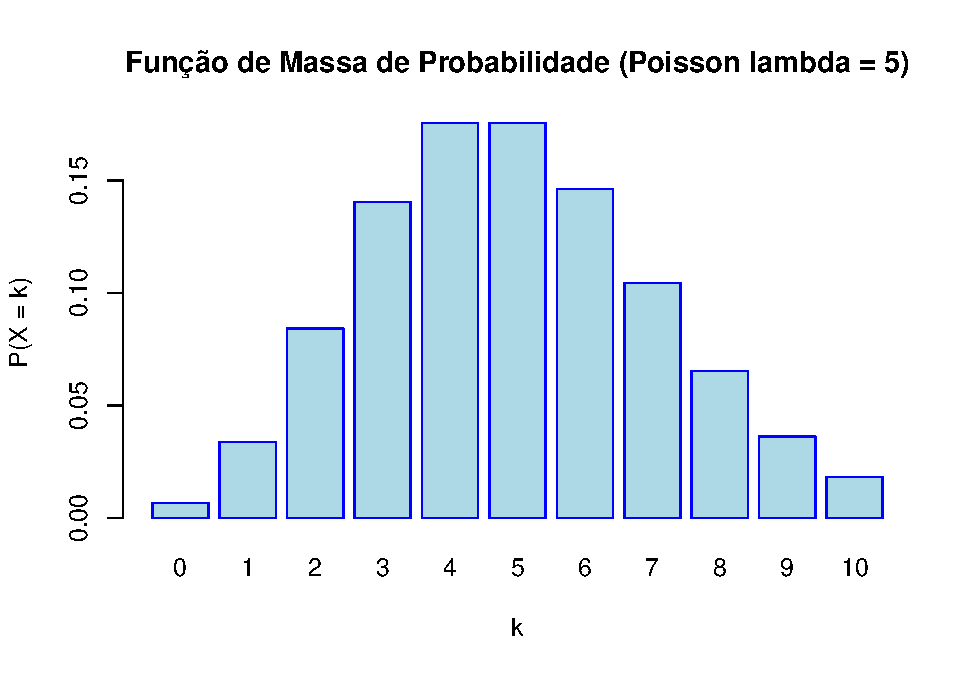
\includegraphics[keepaspectratio]{ex_gerais_files/figure-latex/unnamed-chunk-33-1.pdf}}

\section{b. da densidade de uma variável
X∼N(90,100).}\label{b.-da-densidade-de-uma-variuxe1vel-xn90100.}

\begin{Shaded}
\begin{Highlighting}[]
\NormalTok{media }\OtherTok{\textless{}{-}} \DecValTok{90}
\NormalTok{desvio }\OtherTok{\textless{}{-}} \DecValTok{10}

\NormalTok{x }\OtherTok{\textless{}{-}} \FunctionTok{seq}\NormalTok{(}\DecValTok{60}\NormalTok{, }\DecValTok{120}\NormalTok{, }\AttributeTok{by =} \FloatTok{0.1}\NormalTok{)}

\NormalTok{densidade }\OtherTok{\textless{}{-}} \FunctionTok{dnorm}\NormalTok{(x, }\AttributeTok{mean =}\NormalTok{ media, }\AttributeTok{sd =}\NormalTok{ desvio)}

\FunctionTok{plot}\NormalTok{(x, densidade, }\AttributeTok{type =} \StringTok{"l"}\NormalTok{, }\AttributeTok{lwd =} \DecValTok{2}\NormalTok{,}
     \AttributeTok{main =} \StringTok{"Função de Densidade da Normal N(90, 100)"}\NormalTok{,}
     \AttributeTok{xlab =} \StringTok{"x"}\NormalTok{, }\AttributeTok{ylab =} \StringTok{"f(x)"}\NormalTok{,}
     \AttributeTok{col =} \StringTok{"darkgreen"}\NormalTok{)}
\end{Highlighting}
\end{Shaded}

\pandocbounded{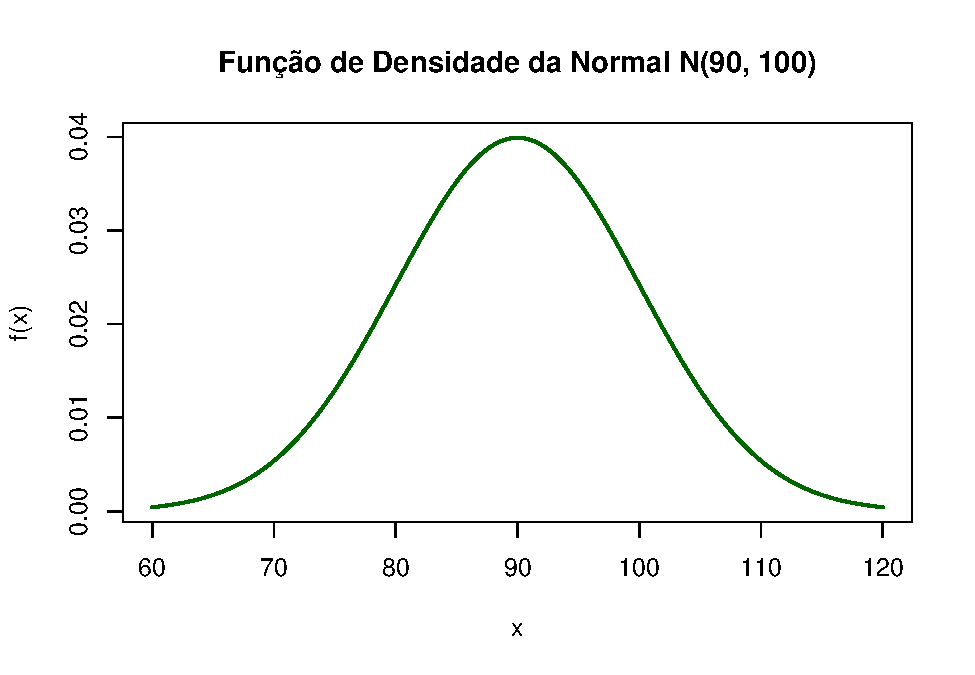
\includegraphics[keepaspectratio]{ex_gerais_files/figure-latex/unnamed-chunk-34-1.pdf}}

\section{c.~sobreponha ao gráfico anterior a densidade de uma variável
Y∼N(90,80) e outra
Z∼N(85,100).}\label{c.-sobreponha-ao-gruxe1fico-anterior-a-densidade-de-uma-variuxe1vel-yn9080-e-outra-zn85100.}

\begin{Shaded}
\begin{Highlighting}[]
\NormalTok{x }\OtherTok{\textless{}{-}} \FunctionTok{seq}\NormalTok{(}\DecValTok{50}\NormalTok{, }\DecValTok{130}\NormalTok{, }\AttributeTok{by =} \FloatTok{0.1}\NormalTok{)}
\NormalTok{densidade\_X }\OtherTok{\textless{}{-}} \FunctionTok{dnorm}\NormalTok{(x, }\AttributeTok{mean =} \DecValTok{90}\NormalTok{, }\AttributeTok{sd =} \FunctionTok{sqrt}\NormalTok{(}\DecValTok{100}\NormalTok{))}
\NormalTok{densidade\_Y }\OtherTok{\textless{}{-}} \FunctionTok{dnorm}\NormalTok{(x, }\AttributeTok{mean =} \DecValTok{90}\NormalTok{, }\AttributeTok{sd =} \FunctionTok{sqrt}\NormalTok{(}\DecValTok{80}\NormalTok{))}
\NormalTok{densidade\_Z }\OtherTok{\textless{}{-}} \FunctionTok{dnorm}\NormalTok{(x, }\AttributeTok{mean =} \DecValTok{85}\NormalTok{, }\AttributeTok{sd =} \FunctionTok{sqrt}\NormalTok{(}\DecValTok{100}\NormalTok{))}

\FunctionTok{plot}\NormalTok{(x, densidade\_X, }\AttributeTok{type =} \StringTok{"l"}\NormalTok{, }\AttributeTok{lwd =} \DecValTok{2}\NormalTok{, }\AttributeTok{col =} \StringTok{"blue"}\NormalTok{,}
     \AttributeTok{ylim =} \FunctionTok{c}\NormalTok{(}\DecValTok{0}\NormalTok{, }\FunctionTok{max}\NormalTok{(densidade\_X, densidade\_Y, densidade\_Z)),}
     \AttributeTok{main =} \StringTok{"Densidades de X \textasciitilde{} N(90,100), Y \textasciitilde{} N(90,80) e Z \textasciitilde{} N(85,100)"}\NormalTok{,}
     \AttributeTok{xlab =} \StringTok{"x"}\NormalTok{, }\AttributeTok{ylab =} \StringTok{"f(x)"}\NormalTok{)}

\FunctionTok{lines}\NormalTok{(x, densidade\_Y, }\AttributeTok{col =} \StringTok{"red"}\NormalTok{, }\AttributeTok{lwd =} \DecValTok{2}\NormalTok{, }\AttributeTok{lty =} \DecValTok{2}\NormalTok{)}
\FunctionTok{lines}\NormalTok{(x, densidade\_Z, }\AttributeTok{col =} \StringTok{"darkgreen"}\NormalTok{, }\AttributeTok{lwd =} \DecValTok{2}\NormalTok{, }\AttributeTok{lty =} \DecValTok{3}\NormalTok{)}
\FunctionTok{legend}\NormalTok{(}\StringTok{"topright"}\NormalTok{, }\AttributeTok{legend =} \FunctionTok{c}\NormalTok{(}\StringTok{"X \textasciitilde{} N(90, 100)"}\NormalTok{, }\StringTok{"Y \textasciitilde{} N(90, 80)"}\NormalTok{, }\StringTok{"Z \textasciitilde{} N(85, 100)"}\NormalTok{),}

       \AttributeTok{col =} \FunctionTok{c}\NormalTok{(}\StringTok{"blue"}\NormalTok{, }\StringTok{"red"}\NormalTok{, }\StringTok{"darkgreen"}\NormalTok{), }\AttributeTok{lwd =} \DecValTok{2}\NormalTok{, }\AttributeTok{lty =} \FunctionTok{c}\NormalTok{(}\DecValTok{1}\NormalTok{, }\DecValTok{2}\NormalTok{, }\DecValTok{3}\NormalTok{))}
\end{Highlighting}
\end{Shaded}

\pandocbounded{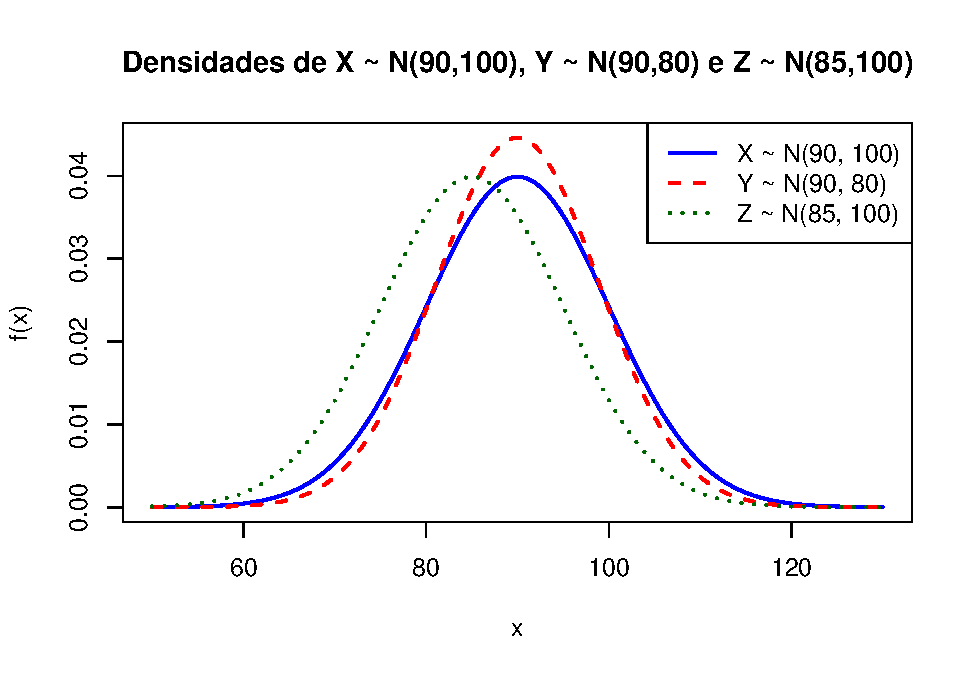
\includegraphics[keepaspectratio]{ex_gerais_files/figure-latex/unnamed-chunk-35-1.pdf}}

\section{\texorpdfstring{d.~densidades de distribuições \(\chi^2\) com
1, 2 e 5 graus de
liberdade.}{d.~densidades de distribuições \textbackslash chi\^{}2 com 1, 2 e 5 graus de liberdade.}}\label{d.-densidades-de-distribuiuxe7uxf5es-chi2-com-1-2-e-5-graus-de-liberdade.}

\begin{Shaded}
\begin{Highlighting}[]
\NormalTok{x }\OtherTok{\textless{}{-}} \FunctionTok{seq}\NormalTok{(}\DecValTok{0}\NormalTok{, }\DecValTok{20}\NormalTok{, }\AttributeTok{by =} \FloatTok{0.1}\NormalTok{)}

\NormalTok{dens\_1 }\OtherTok{\textless{}{-}} \FunctionTok{dchisq}\NormalTok{(x, }\AttributeTok{df =} \DecValTok{1}\NormalTok{)}
\NormalTok{dens\_2 }\OtherTok{\textless{}{-}} \FunctionTok{dchisq}\NormalTok{(x, }\AttributeTok{df =} \DecValTok{2}\NormalTok{)}
\NormalTok{dens\_5 }\OtherTok{\textless{}{-}} \FunctionTok{dchisq}\NormalTok{(x, }\AttributeTok{df =} \DecValTok{5}\NormalTok{)}


\NormalTok{all\_dens }\OtherTok{\textless{}{-}} \FunctionTok{c}\NormalTok{(dens\_1, dens\_2, dens\_5)}
\NormalTok{all\_dens }\OtherTok{\textless{}{-}}\NormalTok{ all\_dens[}\FunctionTok{is.finite}\NormalTok{(all\_dens)]}

\FunctionTok{plot}\NormalTok{(x, dens\_1, }\AttributeTok{type =} \StringTok{"l"}\NormalTok{, }\AttributeTok{lwd =} \DecValTok{2}\NormalTok{, }\AttributeTok{col =} \StringTok{"blue"}\NormalTok{,}
     \AttributeTok{ylim =} \FunctionTok{c}\NormalTok{(}\DecValTok{0}\NormalTok{, }\FunctionTok{max}\NormalTok{(all\_dens)),}
     \AttributeTok{main =} \StringTok{"Densidades da distribuição X\^{}2 com 1, 2 e 5 graus de liberdade"}\NormalTok{,}
     \AttributeTok{xlab =} \StringTok{"x"}\NormalTok{, }\AttributeTok{ylab =} \StringTok{"f(x)"}\NormalTok{)}


\FunctionTok{lines}\NormalTok{(x, dens\_2, }\AttributeTok{col =} \StringTok{"red"}\NormalTok{, }\AttributeTok{lwd =} \DecValTok{2}\NormalTok{, }\AttributeTok{lty =} \DecValTok{2}\NormalTok{)}
\FunctionTok{lines}\NormalTok{(x, dens\_5, }\AttributeTok{col =} \StringTok{"darkgreen"}\NormalTok{, }\AttributeTok{lwd =} \DecValTok{2}\NormalTok{, }\AttributeTok{lty =} \DecValTok{3}\NormalTok{)}

\FunctionTok{legend}\NormalTok{(}\StringTok{"topright"}\NormalTok{, }\AttributeTok{legend =} \FunctionTok{c}\NormalTok{(}\StringTok{"X\^{}2(1)"}\NormalTok{, }\StringTok{"X\^{}2(2)"}\NormalTok{, }\StringTok{"X\^{}2(5)"}\NormalTok{),}
       \AttributeTok{col =} \FunctionTok{c}\NormalTok{(}\StringTok{"blue"}\NormalTok{, }\StringTok{"red"}\NormalTok{, }\StringTok{"darkgreen"}\NormalTok{), }\AttributeTok{lwd =} \DecValTok{2}\NormalTok{, }\AttributeTok{lty =} \FunctionTok{c}\NormalTok{(}\DecValTok{1}\NormalTok{, }\DecValTok{2}\NormalTok{, }\DecValTok{3}\NormalTok{))}
\end{Highlighting}
\end{Shaded}

\pandocbounded{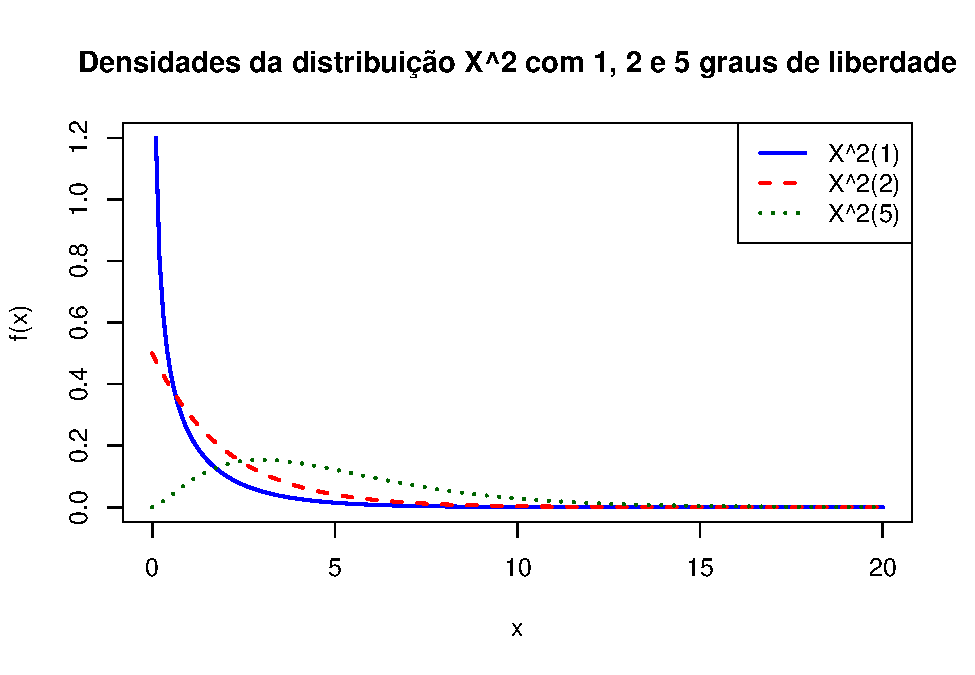
\includegraphics[keepaspectratio]{ex_gerais_files/figure-latex/unnamed-chunk-36-1.pdf}}

\section{Parte 3}\label{parte-3}

\section{Implemente o gerador Midsquare idealizado pelo matemático John
von Neumann. Por que o gerador Midsquare não é um bom gerador?
Explique}\label{implemente-o-gerador-midsquare-idealizado-pelo-matemuxe1tico-john-von-neumann.-por-que-o-gerador-midsquare-nuxe3o-uxe9-um-bom-gerador-explique}

\subsubsection{Implemente o gerador Midsquare idealizado pelo matemático
John von
Neumann.}\label{implemente-o-gerador-midsquare-idealizado-pelo-matemuxe1tico-john-von-neumann.}

\begin{itemize}
\tightlist
\item
  A ideia de início era gerar um n manualmente, mas o rmd nao permite
  isso.
\end{itemize}

\begin{Shaded}
\begin{Highlighting}[]
\NormalTok{gerador\_midsquare }\OtherTok{\textless{}{-}} \ControlFlowTok{function}\NormalTok{(semente, }\AttributeTok{n =} \DecValTok{10}\NormalTok{) \{}

  \CommentTok{\#n \textless{}{-} as.integer(readline(prompt = "Quantos números aleatórios deseja gerar? "))}

\NormalTok{  numeros\_novos }\OtherTok{\textless{}{-}} \FunctionTok{numeric}\NormalTok{(n)}

  \ControlFlowTok{for}\NormalTok{ (i }\ControlFlowTok{in} \DecValTok{1}\SpecialCharTok{:}\NormalTok{n) \{}
\NormalTok{    semente }\OtherTok{\textless{}{-}}\NormalTok{ semente}\SpecialCharTok{\^{}}\DecValTok{2}

\NormalTok{    semente\_str }\OtherTok{\textless{}{-}} \FunctionTok{sprintf}\NormalTok{(}\StringTok{"\%08d"}\NormalTok{, semente)}

\NormalTok{    semente }\OtherTok{\textless{}{-}} \FunctionTok{as.integer}\NormalTok{(}\FunctionTok{substr}\NormalTok{(semente\_str, }\DecValTok{3}\NormalTok{, }\DecValTok{6}\NormalTok{))}

\NormalTok{    numeros\_novos[i] }\OtherTok{\textless{}{-}}\NormalTok{ semente}
\NormalTok{  \}}

  \FunctionTok{return}\NormalTok{(numeros\_novos)}
\NormalTok{\}}



\NormalTok{semente\_inicial }\OtherTok{\textless{}{-}} \FunctionTok{sample}\NormalTok{(}\DecValTok{1000}\SpecialCharTok{:}\DecValTok{9999}\NormalTok{, }\DecValTok{1}\NormalTok{)}
\NormalTok{numeros\_gerados }\OtherTok{\textless{}{-}} \FunctionTok{gerador\_midsquare}\NormalTok{(semente\_inicial, }\AttributeTok{n =} \DecValTok{10}\NormalTok{)}
\FunctionTok{print}\NormalTok{(numeros\_gerados)}
\end{Highlighting}
\end{Shaded}

\begin{verbatim}
##  [1] 7710 4441 7224 1861 4633 4646 5853 2576 6357 4114
\end{verbatim}

\subsubsection{Por que o gerador Midsquare não é um bom
gerador?}\label{por-que-o-gerador-midsquare-nuxe3o-uxe9-um-bom-gerador}

\begin{itemize}
\tightlist
\item
  Ele nao e um bom gerador porque pode gerar sequências de números que
  não são uniformemente distribuídas, especialmente se a semente inicial
  não for escolhida adequadamente. O gerador Midsquare utiliza o
  quadrado da semente e extrai os dígitos do meio, o que pode levar a
  padrões repetitivos. Além disso, ele pode ter um período curto, o que
  significa que os números gerados podem se repetir rapidamente.
\end{itemize}

\end{document}
